% Options for packages loaded elsewhere
\PassOptionsToPackage{unicode}{hyperref}
\PassOptionsToPackage{hyphens}{url}
%
\documentclass[
  12pt,
  ignorenonframetext,
  aspectratio=169]{beamer}
\usepackage{pgfpages}
\setbeamertemplate{caption}[numbered]
\setbeamertemplate{caption label separator}{: }
\setbeamercolor{caption name}{fg=normal text.fg}
\beamertemplatenavigationsymbolsempty
% Prevent slide breaks in the middle of a paragraph
\widowpenalties 1 10000
\raggedbottom
\setbeamertemplate{part page}{
  \centering
  \begin{beamercolorbox}[sep=16pt,center]{part title}
    \usebeamerfont{part title}\insertpart\par
  \end{beamercolorbox}
}
\setbeamertemplate{section page}{
  \centering
  \begin{beamercolorbox}[sep=12pt,center]{part title}
    \usebeamerfont{section title}\insertsection\par
  \end{beamercolorbox}
}
\setbeamertemplate{subsection page}{
  \centering
  \begin{beamercolorbox}[sep=8pt,center]{part title}
    \usebeamerfont{subsection title}\insertsubsection\par
  \end{beamercolorbox}
}
\AtBeginPart{
  \frame{\partpage}
}
\AtBeginSection{
  \ifbibliography
  \else
    \frame{\sectionpage}
  \fi
}
\AtBeginSubsection{
  \frame{\subsectionpage}
}
\usepackage{lmodern}
\usepackage{amsmath}
\usepackage{ifxetex,ifluatex}
\ifnum 0\ifxetex 1\fi\ifluatex 1\fi=0 % if pdftex
  \usepackage[T1]{fontenc}
  \usepackage[utf8]{inputenc}
  \usepackage{textcomp} % provide euro and other symbols
  \usepackage{amssymb}
\else % if luatex or xetex
  \usepackage{unicode-math}
  \defaultfontfeatures{Scale=MatchLowercase}
  \defaultfontfeatures[\rmfamily]{Ligatures=TeX,Scale=1}
\fi
% Use upquote if available, for straight quotes in verbatim environments
\IfFileExists{upquote.sty}{\usepackage{upquote}}{}
\IfFileExists{microtype.sty}{% use microtype if available
  \usepackage[]{microtype}
  \UseMicrotypeSet[protrusion]{basicmath} % disable protrusion for tt fonts
}{}
\makeatletter
\@ifundefined{KOMAClassName}{% if non-KOMA class
  \IfFileExists{parskip.sty}{%
    \usepackage{parskip}
  }{% else
    \setlength{\parindent}{0pt}
    \setlength{\parskip}{6pt plus 2pt minus 1pt}}
}{% if KOMA class
  \KOMAoptions{parskip=half}}
\makeatother
\usepackage{xcolor}
\IfFileExists{xurl.sty}{\usepackage{xurl}}{} % add URL line breaks if available
\IfFileExists{bookmark.sty}{\usepackage{bookmark}}{\usepackage{hyperref}}
\hypersetup{
  pdftitle={INFERÊNCIA CAUSAL COM MACHINE LEARNING},
  pdfauthor={Rafael Felipe Bressan},
  hidelinks,
  pdfcreator={LaTeX via pandoc}}
\urlstyle{same} % disable monospaced font for URLs
\newif\ifbibliography
\setlength{\emergencystretch}{3em} % prevent overfull lines
\providecommand{\tightlist}{%
  \setlength{\itemsep}{0pt}\setlength{\parskip}{0pt}}
\setcounter{secnumdepth}{-\maxdimen} % remove section numbering
\mode<presentation> {
  \usetheme[block=fill]{metropolis}
}

%%% FGV colors for metropolis
% As cores vou deixar definido, estão certas as
% cores da FGV. Só saber como usar agora
\definecolor{brunoblue}{HTML}{182936}
\definecolor{brunomarroon}{HTML}{704730}
\definecolor{brunolightgray}{HTML}{E6E6E6}
\definecolor{fgvblue}{HTML}{1C2F67}
\definecolor{fgvlightblue}{HTML}{0096D6}

% Structure
% \setbeamercolor{structure}{fg=fgvblue}
\setbeamercolor{normal text}{fg=fgvblue}
% \setbeamercolor{separator}{fg=brunomarroon, bg=brunomarroon}
% \setbeamercolor{footline}{bg=fgvlightblue}

% % Blocs
% \setbeamercolor{block body}{bg=brunolightgray}
% \setbeamercolor{block title}{bg=fgvblue, fg=white} 

% Math font
\usepackage{unicode-math}
\usepackage{FiraSans}
\setmainfont{Fira Sans Light}
% \setmathfont{STIX Two Math}

% \usetheme{Bruno}
% \background{fig/FGV-Logo_small.png}
\usepackage{booktabs}
\usepackage{threeparttablex}

% novos comandos
\newcommand{\bfx}{\mathbf{X}}
\newcommand{\bfw}{\mathbf{W}}
\DeclareMathOperator*{\argmin}{argmin}
\ifluatex
  \usepackage{selnolig}  % disable illegal ligatures
\fi
\newlength{\cslhangindent}
\setlength{\cslhangindent}{1.5em}
\newlength{\csllabelwidth}
\setlength{\csllabelwidth}{3em}
\newenvironment{CSLReferences}[2] % #1 hanging-ident, #2 entry spacing
 {% don't indent paragraphs
  \setlength{\parindent}{0pt}
  % turn on hanging indent if param 1 is 1
  \ifodd #1 \everypar{\setlength{\hangindent}{\cslhangindent}}\ignorespaces\fi
  % set entry spacing
  \ifnum #2 > 0
  \setlength{\parskip}{#2\baselineskip}
  \fi
 }%
 {}
\usepackage{calc}
\newcommand{\CSLBlock}[1]{#1\hfill\break}
\newcommand{\CSLLeftMargin}[1]{\parbox[t]{\csllabelwidth}{#1}}
\newcommand{\CSLRightInline}[1]{\parbox[t]{\linewidth - \csllabelwidth}{#1}\break}
\newcommand{\CSLIndent}[1]{\hspace{\cslhangindent}#1}

\title{INFERÊNCIA CAUSAL COM MACHINE LEARNING}
\subtitle{uma aplicação para evasão fiscal}
\author{Rafael Felipe Bressan}
\date{2021-03-14}
\institute{Receita Federal do Brasil}

\begin{document}
\frame{\titlepage}

\hypertarget{motivacao}{%
\section{Motivação}\label{motivacao}}

\begin{frame}{Causalidade}
\protect\hypertarget{causalidade}{}
\begin{itemize}
\item
  Limite de velocidade reduz as mortes no trânsito?
\item
  Permissão para cobrança de bagagem aérea reduziu o preço das tarifas?
\item
  O recebimento de uma carta-cobrança da Receita Federal faz com que o
  contribuinte recolha seus impostos devidos?
\item
  Essas questões são \textbf{causais} em sua natureza. Requerem
  conhecimento do processo de geração dos dados. Suas respostas não
  podem ser calculadas apenas com os dados observados.
\end{itemize}
\end{frame}

\begin{frame}{Causalidade}
\protect\hypertarget{causalidade-1}{}
\begin{itemize}
\item
  Análise causal requer manipulação/intervenção no processo gerador
\item
  Uma quebra estrutural é induzida
\item
  Correlações anteriores não são mais válidas
\item
  Dados puramente observacionais não carregam toda a informação
  necessária
\end{itemize}
\end{frame}

\begin{frame}{\emph{Machine Learning sem Viés}}
\protect\hypertarget{machine-learning-sem-viuxe9s}{}
\[Y_i=f(\mathbf{X}_i, \epsilon_i;\theta)\] - Causalidade requer
inferência sobre parâmetros da distribuição, \(\theta\)

\begin{itemize}
\item
  \emph{Machine Learning} tradicional oferece correlações a partir de
  dados observacionais
\item
  Inferência \(\neq\) previsão

  \begin{itemize}
  \tightlist
  \item
    ML: minimiza \(\hat e = \hat y - Y\)
  \item
    Análise causal: estima \(\hat\theta\) com intervalo de confiança
  \end{itemize}
\item
  Boa previsão \textbf{não garante} correta estimação de parâmetros
\item
  \textcolor{red}{Viés de regularização}:
  \(\hat f_1(\cdot;\hat\theta_1)\approx \hat f_2(\cdot;\hat\theta_2)\)
  mesmo se \(\hat\theta_1\neq\hat\theta_2\)
\end{itemize}
\end{frame}

\begin{frame}{\emph{Machine Learning sem Viés}}
\protect\hypertarget{machine-learning-sem-viuxe9s-1}{}
\begin{itemize}
\item
  Como fazer com que algoritmos de ML façam estimação causal
  não-viesada?
\item
  Fronteira do conhecimento em inferência causal

  \begin{itemize}
  \tightlist
  \item
    Chernozhukov et al. (2018) - \emph{Double Machine Learning}
  \item
    Wager and Athey (2018) - \emph{Causal Forests}
  \item
    Syrgkanis et al. (2019) - \emph{Doubly Robust Instrumental
    Variables}
  \end{itemize}
\end{itemize}
\end{frame}

\hypertarget{experimento}{%
\section{Experimento Randomizado}\label{experimento}}

\begin{frame}{Experimento Randomizado}
\protect\hypertarget{experimento-randomizado}{}
\begin{itemize}
\item
  Experimentos randomizados são o padrão-ouro para inferência causal
\item
  Re-analisaremos o trabalho de Fellner, Sausgruber, and Traxler (2013)
\item
  Correspondências fiscais para mais de 50.000 contribuintes
\item
  Analisar efeitos de variação no conteúdo

  \begin{itemize}
  \tightlist
  \item
    Valores médios por tipo de carta
  \item
    Heterogeneidade nos efeitos
  \end{itemize}
\end{itemize}
\end{frame}

\begin{frame}{Descrição do Experimento}
\protect\hypertarget{descriuxe7uxe3o-do-experimento}{}
\begin{table}[H]

\centering
\begin{tabular}[t]{llrr}
\toprule
Tratamento & Descrição & Observações & Proporção\\
\midrule
T0 & Sem Correio & 2586 & 0.0512099\\
T1 & Correio & 7984 & 0.1581053\\
T2 & Ameaça & 7821 & 0.1548774\\
T3 & Info & 7998 & 0.1583825\\
T4 & Info\&Ameaça & 8101 & 0.1604222\\
T5 & Moral & 8084 & 0.1600855\\
T6 & Moral\&Ameaça & 7924 & 0.1569171\\
\bottomrule
\end{tabular}
\end{table}
\end{frame}

\begin{frame}{Problema de Atrito}
\protect\hypertarget{problema-de-atrito}{}
\begin{itemize}
\tightlist
\item
  Atrito: contribuintes que deveriam receber a correspondência mas não
  foram encontrados
\item
  Pode comprometer a aleatorização do experimento e \textbf{gerar viés}
  na inferência
\end{itemize}

\begin{table}[H]
\centering
\begin{threeparttable}
\footnotesize
\begin{tabular}[t]{llrrr}

\toprule
Tratamento & Descrição & Cartas & Não Entregues & Taxa Atrito\\
\midrule
T1 & Correio & 7984 &  1126 & 0.1410\\
T2 & Ameaça & 7821 &  1127 & 0.1441\\
T3 & Info & 7998 &  1173 & 0.1467\\
T4 & Info\&Ameaça & 8101 &  1141 & 0.1408\\
T5 & Moral & 8084 &  1164 & 0.1440\\
\addlinespace
T6 & Moral\&Ameaça & 7924 & 1174 & 0.1482\\
\bottomrule
\end{tabular}
\end{threeparttable}
\end{table}
\end{frame}

\begin{frame}{Análise Exploratória}
\protect\hypertarget{anuxe1lise-exploratuxf3ria}{}
\begin{itemize}
\tightlist
\item
  Uma boa aleatorização implica em balanceamento das covariadas
  \emph{(features)} entre os tratamentos
\end{itemize}

\begin{table}[H]
\centering
\fontsize{8}{10}\selectfont
\begin{threeparttable}
\begin{tabular}[t]{llrrrrrr}
\toprule
Tratamento & Descrição & Gênero & Idade & Renda & População & Dens. pop. & Compliance\\
\midrule
T0 & Sem Correio & 0.6458 & 48.0170 & 20928.4068 & 45815.2715 & 8.1711 & 0.9355\\
T1 & Correio & 0.6338 & 47.9969 & 20878.9958 & 43377.1935 & 8.5625 & 0.9352\\
T2 & Ameaça & 0.6367 & 47.9931 & 20901.1614 & 44542.5883 & 7.9605 & 0.9346\\
T3 & Info & 0.6260 & 48.0300 & 20882.6636 & 43903.0189 & 8.1142 & 0.9347\\
T4 & Info\&Ameaça & 0.6335 & 48.0051 & 20879.6138 & 43319.4736 & 8.3540 & 0.9352\\
\addlinespace
T5 & Moral & 0.6251 & 47.9982 & 20888.4584 & 44301.3718 & 8.4832 & 0.9343\\
T6 & Moral\&Ameaça & 0.6422 & 47.9904 & 20876.3062 & 43610.1972 & 8.0468 & 0.9343\\
\midrule
Anova: & p-values & 0.1715 & 0.3993 & 0.9393 & 0.7577 & 0.5795 & 0.8614\\
\bottomrule
\end{tabular}
\end{threeparttable}
\end{table}
\end{frame}

\begin{frame}{Análise Exploratória}
\protect\hypertarget{anuxe1lise-exploratuxf3ria-1}{}
\begin{itemize}
\tightlist
\item
  Atrito pode quebrar o balanceamento e comprometer a aleatorização
\end{itemize}

\begin{table}[H]
\centering
\fontsize{8}{10}\selectfont
\begin{threeparttable}
\begin{tabular}[t]{lrrrrrr}
\toprule
Tratamento & Gênero & Idade & Renda & População & Dens. pop. & Compliance\\
\midrule
T0 & 0.6458 & 48.0170 & 20928.4068 & 45815.2715 & 8.1711 & 0.9355\\
T1 & 0.6403 & 47.7868 & 21100.3921 & 52084.9822 & 7.6001 & 0.9322\\
T2 & 0.6211 & 47.7127 & 21106.0117 & 48882.0302 & 6.5860 & 0.9337\\
T3 & 0.6138 & 47.8580 & 21077.8894 & 51027.8338 & 6.6317 & 0.9313\\
T4 & 0.6240 & 47.8056 & 20945.2352 & 48251.5259 & 6.5957 & 0.9318\\
\addlinespace
T5 & 0.6177 & 47.7952 & 20864.3756 & 43273.7019 & 6.3919 & 0.9308\\
T6 & 0.6320 & 47.8117 & 20966.9995 & 46539.3467 & 6.4614 & 0.9324\\
\midrule
Anova p-valor & 0.4319 & 0.0000 & 0.0095 & 0.0936 & 0.0094 & 0.1122\\
\bottomrule
\end{tabular}
\end{threeparttable}
\end{table}
\end{frame}

\hypertarget{modelos-e-resultados}{%
\section{Modelos e Resultados}\label{modelos-e-resultados}}

\begin{frame}{Estimandos Causais}
\protect\hypertarget{estimandos-causais}{}
\begin{itemize}
\tightlist
\item
  \emph{Framework} de Resultados potenciais. Observamos apenas um
  resultado potencial dado um tratamento.
  \textcolor{red}{Problema fundamental da inferência causal}
\end{itemize}

\[Y_i=D_i\cdot Y_i(1)+(1-D_i)\cdot Y_i(0), \quad D_i\in\{0, 1\}\]

\begin{itemize}
\tightlist
\item
  Estimandos Casusais:
\end{itemize}

\vspace{-1em}

\begin{align*}
    ATE&=\mathbb{E}[Y_i(1)-Y_i(0)], \qquad\qquad\, CATE(x)=\mathbb{E}[Y_i(1)-Y_i(0)|\mathbf{X}=x]\\
    ATT&=\mathbb{E}[Y_i(1)-Y_i(0)|D_i=1], \quad CATT(x)=\mathbb{E}[Y_i(1)-Y_i(0)|\mathbf{X}=x, D_i=1]\\
     LAT&E(x)=\frac{\mathbb{E}[Y_i(1, D_i(1))-Y_i(0, D_i(0))]}{\mathbb{E}[D_i(1)-D_i(0)]}
\end{align*}
\end{frame}

\begin{frame}{Hipóteses de Identificação}
\protect\hypertarget{hipuxf3teses-de-identificauxe7uxe3o}{}
\begin{itemize}
\item
  SUTVA: \textbf{não existe interferência} entre os indivíduos tratados
  e não tratados. Não pode haver efeitos de transbordamento do
  tratamento de algum indivíduo para outro que esteja no grupo de
  controle
\item
  CIA \emph{(unconfoundedness)}: \textbf{condicionado às características
  observadas}, \(\mathbf{X}_i\), os resultados potenciais são
  \textbf{independentes} do tratamento \(D_i\),
  \(\{Y_i(1), Y_i(0)\} \perp D_i|\mathbf{X}_i\)
\end{itemize}

Quando usamos variáveis instrumentais

\begin{itemize}
\item
  Exclusão do instrumento: designação para tratamento \textbf{não afeta
  diretamente} os resultados potenciais
\item
  Relevância do instrumento: designação para o tratamento aumenta a
  probabilidade de ser tratado. \(\mathbb{E}[D_i(1)-D_i(0)]>0\)
\end{itemize}
\end{frame}

\begin{frame}{Modelo ForestDML}
\protect\hypertarget{modelo-forestdml}{}
\begin{itemize}
\tightlist
\item
  Modelo parcialmente linear. Tratamento \(T\) é exógeno, não é
  necessária instrumentalização
\end{itemize}

\vspace{-1em}

\begin{align*}
    Y&=\theta(\bfx) \cdot T+g(\bfx, \bfw)+\epsilon  &\mathbb{E}[\epsilon \mid \bfx, \bfw]=0 \\
    T&=f(\bfx, \bfw)+\eta &\mathbb{E}[\eta \mid \bfx, \bfw]=0 \\
    \mathbb{E}&[\eta \cdot \epsilon \mid \bfx, \bfw]=0
\end{align*}

\begin{itemize}
\tightlist
\item
  Através de \textcolor{red}{DML} (ortogonalização de Neyman e
  \emph{cross-fitting})
\end{itemize}

\vspace{-1em}

\begin{equation*}
\hat{\theta}(x)=\argmin_{\theta} \sum_{i=1}^{n} K_{x}\left(X_{i}\right) \cdot\left(Y_{i}-\hat{q}\left(X_{i}, W_{i}\right)-\theta \cdot\left(T_{i}-\hat{f}\left(X_{i}, W_{i}\right)\right)\right)^{2}
\end{equation*}

\begin{itemize}
\tightlist
\item
  \emph{Kernel} \(K_x\) é uma \textcolor{red}{floresta causal}
\end{itemize}
\end{frame}

\begin{frame}{Modelo DRIV}
\protect\hypertarget{modelo-driv}{}
\begin{itemize}
\tightlist
\item
  Tratamento é endógeno. Necessita de variável instrumental
\end{itemize}

\vspace{-1em}

\begin{align*}
    Y&=\theta(\bfx)\cdot T+g(\bfx)+\epsilon, &\mathbb{E}[\epsilon\mid \bfx, Z]=0\\
    Z&=m(\bfx)+\eta, &\mathbb{E}[\eta\mid\bfx]=0\\
    \mathbb{E}&[\eta\cdot\epsilon\mid \bfx, Z]=0\\
    \mathbb{E}&[T\cdot\epsilon\mid\bfx]\neq 0
\end{align*}

\begin{itemize}
\tightlist
\item
  Estimativa preliminar de \(\theta(x)\) e algoritmo \emph{Doubly
  Robust}
\end{itemize}

\vspace{-1em}

\begin{equation*}
\hat{\theta}_{DR}(x)=\argmin_{\theta}\sum_{i\in\mathcal{I}}\left(\theta_{\text {pre }}(x)+\frac{\left(\hat{\tilde{Y}}_i-\theta_{\text {pre }}(x) \hat{\tilde{T}}_i\right) \hat{\tilde{Z}}_i}{\hat\beta(X_i)}-\theta(X_i)\right)^{2}
\end{equation*}
\end{frame}

\begin{frame}{Resultados}
\protect\hypertarget{resultados}{}
\begin{itemize}
\tightlist
\item
  Receber uma correspondência \textcolor{red}{tem efeito positivo} sobre
  o registro para pagamento do tributo
\item
  Uma \textbf{ameaça} na carta aumenta este efeito
\item
  Informações e apelo moral não possui efeito estatisticamente
  significativo
\end{itemize}

\begin{table}[H]
\centering
\fontsize{8}{10}\selectfont
\begin{tabular}{lccccc}
\toprule\toprule
 & OLS & \multicolumn{2}{c}{ForestDML} & IV2SLS &   DRIV \\
% \cmidrule{2-3}\cmidrule{4}\cmidrule{5}\\
 &    ATE &   ATE &    ATT &   LATE &   LATE \\
\midrule
Correio & 0,0650  & 0,0766 & 0,0766 & 0,0767 & 0,0588 \\
\textbf{Ameaça}  & \textbf{0,0750}  & \textbf{0,0850} & \textbf{0,0848} & \textbf{0,0872} & \textbf{0,0650} \\
Info    & 0,0646  & 0,0762 & 0,0760 & 0,0728 & 0,0547 \\
Moral   & 0,0648  & 0,0695 & 0,0695 & 0,0724 & 0,0513 \\
\bottomrule\bottomrule
\end{tabular}
\end{table}
\end{frame}

\begin{frame}{Efeitos Heterogêneos}
\protect\hypertarget{efeitos-heteroguxeaneos}{}
\begin{itemize}
\tightlist
\item
  Existem características que moderam o efeito causal?
\item
  Heterogeneidade: efeito causal depende de características individuais
\item
  Regressão linear

  \begin{itemize}
  \tightlist
  \item
    \textcolor{green}{Simples estimação e interpretação}
  \item
    \textcolor{red}{Hipótese a priori das características}
  \end{itemize}
\item
  \emph{Machine Learning}

  \begin{itemize}
  \tightlist
  \item
    \textcolor{green}{descobre a heterogeneidade presente nos dados}
  \item
    \textcolor{red}{modelos mais complexos}
  \end{itemize}
\item
  Árvores de decisão são um bom compromisso. Aliam interpretabilidade
  com algoritmo \emph{data-driven}
\end{itemize}
\end{frame}

\begin{frame}
\begin{center}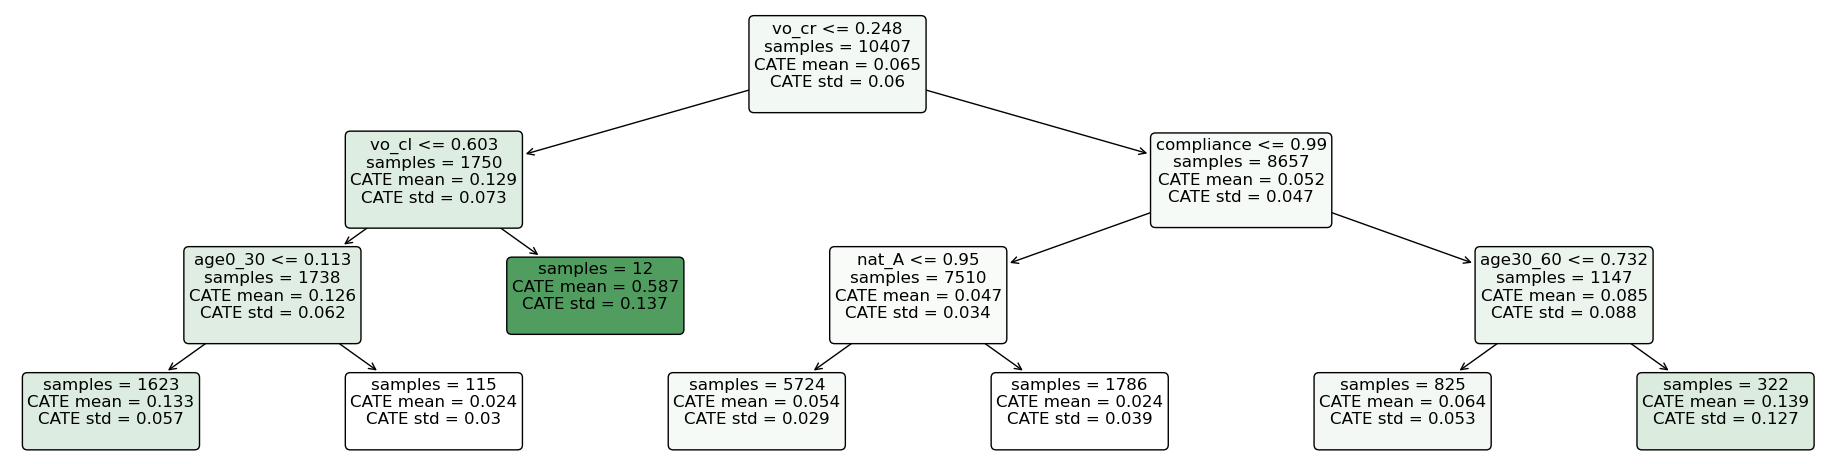
\includegraphics[width=400px]{Figs/fig_tree_driv_cut} \end{center}
\end{frame}

\hypertarget{conclusuxe3o}{%
\section{Conclusão}\label{conclusuxe3o}}

\begin{frame}{Conclusão}
\begin{itemize}
\item
  Árvores de decisão são de fácil interpretação. Conjunto de regras
\item
  Fornece informação sobre as características mais relevantes para
  detectar efeitos heterogêneos
\item
  Os métodos de DML e Causal Forests estimam efeitos livres de viés,
  heterogêneos e não-paramétricos
\item
  Com base nestas estimações, uma \textbf{política ótima} de tratamento
  pode ser implementada, focando nos indivíduos com maior potencial de
  resposta
\end{itemize}
\end{frame}

\begin{frame}[allowframebreaks]{Referências}
\protect\hypertarget{referuxeancias}{}
\scriptsize

\hypertarget{refs}{}
\begin{CSLReferences}{1}{0}
\leavevmode\hypertarget{ref-Chernozhukov2018}{}%
Chernozhukov, Victor, Denis Chetverikov, Mert Demirer, Esther Duflo,
Christian Hansen, Whitney Newey, and James Robins. 2018.
{``{Double/debiased machine learning for treatment and structural
parameters}.''} \emph{The Econometrics Journal} 21 (1): C1--68.
\url{https://doi.org/10.1111/ectj.12097}.

\leavevmode\hypertarget{ref-Fellner2013}{}%
Fellner, Gerlinde, Rupert Sausgruber, and Christian Traxler. 2013.
{``Testing Enforcement Strategies in the Field: Threat, Moral Appeal and
Social Information.''} \emph{Journal of the European Economic
Association} 11 (3): 634--60.

\leavevmode\hypertarget{ref-Syrgkanis2019}{}%
Syrgkanis, Vasilis, Victor Lei, Miruna Oprescu, Maggie Hei, Keith
Battocchi, and Greg Lewis. 2019. {``Machine Learning Estimation of
Heterogeneous Treatment Effects with Instruments.''}
\url{http://arxiv.org/abs/1905.10176}.

\leavevmode\hypertarget{ref-Wager2018}{}%
Wager, Stefan, and Susan Athey. 2018. {``Estimation and Inference of
Heterogeneous Treatment Effects Using Random Forests.''} \emph{Journal
of the American Statistical Association} 113 (523): 1228--42.

\end{CSLReferences}
\end{frame}

\end{document}
